\section{Apache Hadoop}\label{sec:hadoop}

\emph{Apache Hadoop} ist ein Open-Source-Software-Projekt, in dem Software für verteilte Systeme entwickelt wird. Hadoop wird von der \emph{Apache Foundation} entwickelt und bietet verschiedene Komponenten an, welche vollständig skalierbar sind, von einer einfachen Installation auf einem PC bis hin zu einer Installation über mehrere Server in einem Serverzentrum. Hadoop besteht hauptsächlich aus folgenden Kernmodulen \cite{HadoopHomePage}:

\begin{description}
	\item[Hadoop Common] Gemeinsam genutzte Kernkomponenten
	\item[Hadoop Distributed File System] Kurz HDFS, Verteiltes Dateisystem
	\item[Hadoop YARN] Framework zur Verteilung und Ausführung von Tasks und das dazugehörige Ressourcen-Management
	\item[Hadoop MapReduce] YARN-Basiertes System zum Verarbeiten von großen Datenmengen
\end{description}

Hadoop ermöglicht es dadurch, sehr einfach mit Tasks umzugehen, welche große Datenmengen verarbeiten. Da es für Hadoop nicht relevant ist, auf wie vielen Servern es läuft, kann es beliebig skaliert werden, wodurch entsprechend viele Ressourcen zur Bearbeitung und Speicherung von großen Datenmengen zur Verfügung stehen können.

\begin{figure}
	\centering
	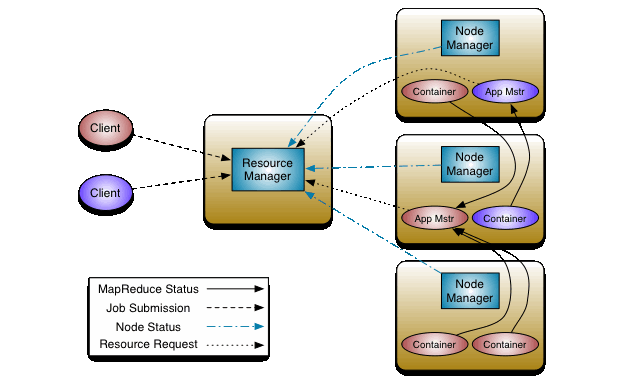
\includegraphics[width=\columnwidth]{./images/yarn_architecture.png}
	\caption[Architektur von YARN]{Architektur von YARN \cite{HadoopYarnDesc272}}
	\label{fig:yarnarch}
\end{figure}

Die Kernidee der Architektur von YARN ist die Trennung vom Ressourcenmanagement und Scheduling. Dazu besitzt der Master den \emph{ResourceManager}, welcher für das gesamte System zuständig ist und die Anwendungen im System überwacht. Er besteht aus zwei Kernkomponenten, dem \emph{ApplicationsManager} und dem \emph{Scheduler}. Der ApplicatonsManager ist für die Annahme und Ausführung von einzelnen Anwendungen zuständig, denen der Scheduler die dafür notwendigen Ressourcen zuteilt und überwacht. Für jeden Slave-\emph{Node} im Hadoop-System gibt es dazu einen \emph{NodeManager}, welcher die lokalen Ressourcen des Nodes überwacht und dem ResourceManager mitteilt. Jede Anwendung besitzt jeweils einen eigenen \emph{ApplicationMaster}, welcher für das Monitoring und die Kommunikation mit dem ResourceManager und NodeManager zuständig ist und die dazu notwendigen Informationen bereit stellt. Jede YARN-Anwendung bzw. Job oder Task besteht zudem aus einem oder mehreren \emph{Containern}, in welchen die Tasks ausgeführt werden. Jeder Bestandteil eines Tasks kann auf jedem beliebigen Node ausgeführt werden \cite{HadoopYarnDesc272}.

\begin{figure}
    \centering
    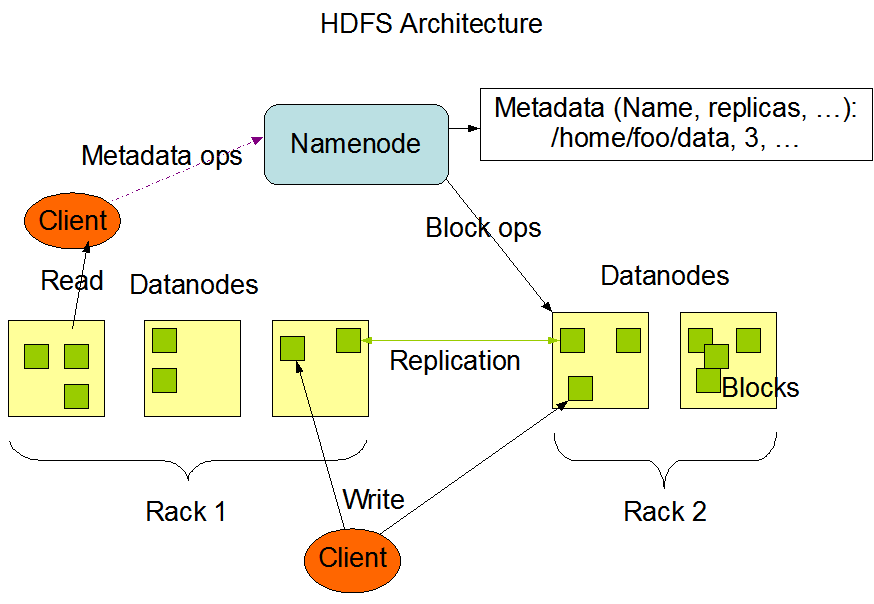
\includegraphics[width=\columnwidth]{./images/hdfsarchitecture.png}
    \caption[Architektur des HDFS]{Architektur des HDFS \cite{HadoopHdfsDesc272}}
    \label{fig:hdfsarch}
\end{figure}

Das HDFS basiert auf der gleichen Architektur wie YARN und besitzt ebenfalls einen Master und mehrere Slaves, welche in der Regel die gleichen Nodes sind wie bei YARN. Der \emph{NameNode} ist als Master für die Verwaltung des Dateisystems zuständig und reguliert den Zugriff auf die darauf gespeicherten Daten. Die Daten selbst werden in mehrere Blöcke aufgeteilt auf den \emph{DataNodes} gespeichert. Um den Zugriff auf die Daten im Falle eines Node-Ausfalls zu gewährleisten, wird jeder Block auf anderen DataNodes repliziert. Dateioperationen (wie Öffnen oder Schließen) werden direkt auf den DataNodes ausgeführt, sie sind darüber hinaus auch dafür verantwortlich, dass Clients die Daten lesen oder beschreiben können \cite{HadoopHdfsDesc272}.

%Hier soll Hadoop in einer modifizierten Variante zum Einsatz kommen. In \cite{zhang2016} haben Zhang et. al. eine Verbesserung des Scheduler des ResourceManagers vorgestellt, welche genutzt werden soll. Im Vergleich zur Standard-Einstellung von Hadoop benötigt diese mit einer selbstadaptiven Komponente ausgestatte Modifikation im Schnitt um bis zu 40 Prozent weniger Zeit zur Ausführung eines Tasks. Dazu wird der zur Verfügung stehende Arbeitsspeicher zur Laufzeit so eingeteilt, damit immer die maximal mögliche Anzahl an Tasks ausgeführt werden können.